\documentclass{article}
\usepackage{geometry}
\geometry{a4paper}
\usepackage{tikz}
\usepackage{xepersian}
\settextfont{XB Niloofar}
\usepackage{bidipoem}
\begin{document}
\centering
مثلاً من دلم می‌خواد یه مثلّث بکشم: \tikz \draw (0,0) -- (1,2) -- (2,0) -- (0,0);
\begin{figure}
	% \begin{center}
	% \centering
	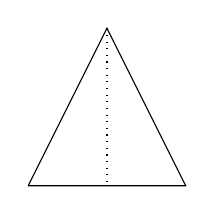
\begin{tikzpicture}
		\draw (0,0) -- (1,2) -- (2,0) -- (0, 0);
		\draw[dotted] (1,2) -- (1,0);
	\end{tikzpicture}
	% \end{center}
	\caption{مثلّث متساوی‌الساقین}
	\label{fig:triangle}
\end{figure}
\end{document}
